% Created 2019-07-13 Sat 17:51
% Intended LaTeX compiler: pdflatex
\documentclass[11pt]{article}
\usepackage[latin1]{inputenc}
\usepackage[T1]{fontenc}
\usepackage{graphicx}
\usepackage{grffile}
\usepackage{longtable}
\usepackage{wrapfig}
\usepackage{rotating}
\usepackage[normalem]{ulem}
\usepackage{amsmath}
\usepackage{textcomp}
\usepackage{amssymb}
\usepackage{capt-of}
\usepackage{hyperref}
\author{Nicolás Luarte}
\date{\today}
\title{Zapata}
\hypersetup{
 pdfauthor={Nicolás Luarte},
 pdftitle={Zapata},
 pdfkeywords={},
 pdfsubject={},
 pdfcreator={Emacs 25.2.2 (Org mode 9.2.3)}, 
 pdflang={English}}
\begin{document}

\maketitle
\tableofcontents

\section{Ciclos}
\label{sec:org55e8c1b}
\subsection{Ciclo 1:}
\label{sec:orgec1628c}
\begin{center}
\begin{tabular}{lll}
Ejercicio & Protocolo & Bloque\\
\hline
Sentadilla de competencia & x1@8, 20\%, 4x5 & A\\
Press banca de competencia & x1@8, 15\%, 4x6 & A\\
Press banca agarre cerrado, pies arriba & x8@9, 10\%, 3x8 & A\\
Press banca con mancuernas & x15@9, 10\%, 3x15 & A\\
\hline
Press banca agarre cerrado & x1@8, 15\%, 4x6 & B\\
Peso muerto de competencia (sumo) & x1@8, 10\%, 4x3 & B\\
Peso muerto hasta las rodillas & x5@8, 3 sets & B\\
Peso muerto bloques & x10@8, 2 sets & B\\
\hline
\end{tabular}
\end{center}

\section{Comentarios t�cnicos}
\label{sec:org7a5e8d6}
\subsection{08/07/2019, ciclo 1, bloque a}
\label{sec:orge78fd0d}
\subsubsection{Sentadilla de competencia}
\label{sec:orgf454269}
\begin{itemize}
\item Fijarse en que el peso este bien balanceado a lo largo de todo el
pie
\item Cambiar la "vocal" del brace de a --> O
\item Inflar los obliquos
\item Luego del unrack, botas aire, haces braces, evita botadas de aire
innecesarias, ya que eso solo va prolongar el comando de bajar
\end{itemize}
\subsubsection{Press banca de competencia}
\label{sec:org595f48d}
\begin{itemize}
\item Llevar activamente el pecho a la barra desde el momento del unrack
\item Los antebrazos no deben tener un ángulo más abierto que 90° respecto
al suelo
\item Para lo anterior intenta tocar un poquito mas arriba en el pecho
\item Imagina que en el pecho llevas un huevo, la barra de parar apenas
tocando el huevo, evita que la barra caiga como saco de papas en tú
pecho, ya que eso romperia el huevo
\end{itemize}

\subsection{09/07/2019, ciclo 1, bloque b}
\label{sec:orgf8b4679}
\subsubsection{Peso muerto de competencia (sumo)}
\label{sec:org0871169}
\begin{itemize}
\item Revisar los gif que te mande para empezar a implementar el setup
"estatico" del que hablamos
\item Tensar la barra hasta que todo este en posicion
\item Una vez tensanda la barra empezar a levantarla del suelo
\item Del suelo a las rodillas extender los menos posible las piernas
\item Una vez la barra toque las rodillas extender agresivamente las
rodillas
\item Cuando este a mitad del muslo, piensa en llevar la cadera
agresivamente hacia adelante
\end{itemize}
\subsubsection{Press banca agarre cerrado}
\label{sec:org73d584d}
\begin{itemize}
\item No me llego video de esto
\end{itemize}

\subsection{12/07/2019, ciclo 1, bloque a}
\label{sec:orgc00226d}
\subsubsection{Sentadilla de competencia}
\label{sec:org39bb73b}
\begin{itemize}
\item Considerar lo comentado en los audios
\item Mantener el cuello hacia 'atr�s' a manera de tenir una postura mas
erguida
\item Walk-out de solo 2 pasos
\item Fijar un punto con la mirada y seguirlo durante todo el
levantamiento, esto tiende a ayudar en el balance significativamente
\end{itemize}
\subsubsection{Press banca de competencia}
\label{sec:org455e469}
\begin{itemize}
\item El orden �ptimo para la banca es (1) brace, (2) unrack, (3)
bajada/subida. Est�s haciendo el brace luego de sacarla, todo el
posicionamiento sucede antes de sacarla y se sostiene. Es mucho m�s
s�lido armarse sin peso en las manos que con peso en las manos
\item Est� mejor la parada el pecho, pero a�n veo que la banca est�
descansando en este, intenta buscar una pausa activa, es decir, que
estes todo el ratos haciendo fuerza en la barra nunca descansas
\item Finalmente, reforzar siempre el arco usando los pilares del rack
\end{itemize}

\subsection{13/07/2019, ciclo 1, bloque b}
\label{sec:orgcc238c2}
\subsubsection{Peso muerto de competencia (sumo)}
\label{sec:org0aa3ba6}
\begin{itemize}
\item Seguir practicando el nuevo setup para sumo
\item Del suelo hasta bajo de las rodillas tu misi�n es mantener la
posici�n los m�s poible sin extender mucho las rodillas
\item Desde las rodillas hasta arriba, busca un bloqueo explosivo
\end{itemize}
\subsubsection{Press banca agarre cerrado}
\label{sec:org5d3075e}
\begin{itemize}
\item Mas tensi�n en el pecho, trata de que la barra apenas si toque el
pecho, nada de hundirla
\item Prueba abrir mas los pies, y forzar mas arco, el objetivo por ahora
sera que las rodillas quede bajo la cresta de tu cadera
\end{itemize}

\section{Registro de progreso}
\label{sec:orgb6fda35}
\begin{center}
\label{tab:orgfc397aa}
\begin{tabular}{lrrl}
Ejercicio & RPE & Peso & Fecha\\
\hline
Sentadilla de competencia & 8 & 175 & 08/07/2019\\
Press banca de competencia & 7.5 & 85 & 08/07/2019\\
Press banca agarre cerrado, pies arriba & nil & nil & 08/07/2019\\
Press banca con mancuernas & nil & nil & 08/07/2019\\
Press banca agarre cerrado & 8 & 80 & 09/07/2019\\
Peso muerto de competencia & 8 & 220 & 09/07/2019\\
Peso muerto hasta las rodillas & 8 & 170 & 09/07/2019\\
Peso muerto bloques & 8 & 120 & 09/07/2019\\
Sentadilla de competencia & 8.5 & 184 & 12/07/2019\\
Press banca de competencia & 8 & 88 & 12/07/2019\\
Press banca agarre cerrado & 8.5 & 85 & 13/07/2019\\
Peso muerto de competencia & 8 & 200 & 13/07/2019\\
Peso muerto hasta las rodillas & 8 & 170 & 13/07/2019\\
Peso muerto bloques & 8 & 120 & 13/07/2019\\
 &  &  & \\
\end{tabular}
\end{center}
\begin{center}
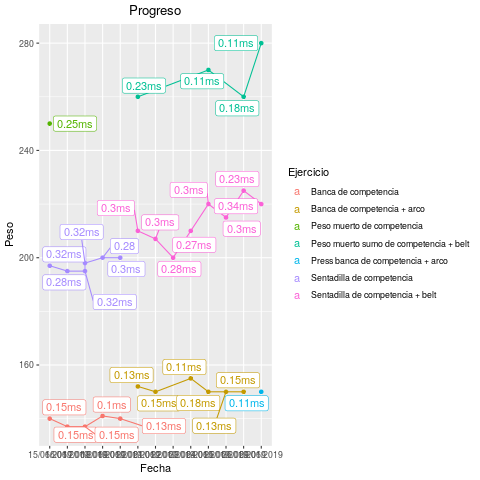
\includegraphics[width=.9\linewidth]{tmp.png}
\end{center}
\end{document}
